Barrier certificates can be used to (in)validate the safety compliance of a controller design by testing if a barrier certificate can be found according to \autoref{eq:barrier_constraints} for the closed-loop system $f_{cl}(x)$. When the vector field of the closed-loop system is polynomial and the sets $\mathcal{X}$, $\mathcal{X}_0$ and $\mathcal{X}_u$ are described by polynomial (in)equalities, a polynomial barrier certificate can be constructed using \gls{sos} optimization \citep{bib:prajna_framework}. A polynomial $p(x)$ is \gls{sos} if there exist polynomials $f_1,\dots,f_m$ such that \citep{bib:parrilo_sdp}
\begin{equation}
p(x) = \sum_{j=1}^{m}f_j^2(x)
\end{equation}

A \gls{sos} program is a convex optimization problem of the form \citep{bib:prajna_framework,bib:sostools}
\begin{subequations}
\begin{align}
&\min_{c}\, w^Tc\\
&\text{subject to} \qquad
q_{i,0}(x) + \sum_{j=1}^{m} q_{i,j}(x)g_j(x) \,\,\,\in \Sigma[x]
\qquad \text{for}\quad
i=1,\dots, p
\end{align}
\end{subequations}
\vspace*{-4mm}
\begin{tabular}{rl}
where &\\
$w$ & is a vector of weighting coefficients of the linear objective function\\
$c$ & is a vector formed by the (unknown) scalar real coefficients of $g_j(x)$\\
$g_j(x)$ & are polynomials in $x$\\
$q_{i,j}(x)$ & are given \gls{sos} polynomials with fixed coefficients\\
$\Sigma$ & denotes the set of \gls{sos} variables\\
$\mathbb{R}[x]$ &denotes a set of polynomials in $x$ with coefficients in $\mathbb{R}$\\
\end{tabular}\\\\


Introducing the notion of a monomial vector as a vector $Z$ in $x$ of degree $deg$; e.g. if $x\in\mathbb{R}^2$ and $deg=[0:2]$ each entry has the form $x_1^ax_2^b$ with exponents $a+b=deg=0,...,2$ i.e.
\begin{equation}
Z=[x_1^0x_2^0\quad x_1^1x_2^0\quad x_1^0x_2^1\quad x_1^1x_2^1\quad x_1^2x_2^0\quad x_1^0x_2^2]^T=[1\quad x_1\quad x_2\quad x_1x_2\quad x_1^2\quad x_2^2]^T
\end{equation} 
Now, according to \citep{bib:parrilo_sdp} a \gls{sos} polynomial $p\in \Sigma[x]$ can be formulated on a quadratic form comprising a coefficient matrix and a monomial vector
\begin{equation}
p = Z^T Q \, Z, \qquad\qquad p\geq 0 \quad \forall \, x\in\mathbb{R}^n %\setminus \{0\}
\label{eq:sos_polynomial}
\end{equation}
\begin{tabular}{rl}
where &\\
$Z$ & is a monomial vector in $x\in \mathbb{R}^n$\\
$Q$ & is a real positive semidefinite symmetric coefficient matrix\\
\end{tabular}\\

Now a polynomial barrier certificate can be constructed using Putinar's Positivstellensatz.
A Positivstellensatz is a structure theorem of a positive polynomial on some set, and gives an algebraic certificate that a solution exists for a system of real polynomial inequalities \citep{bib:positivstellensatz}. 
%Obtain certificates of positivity on a basic semialgebraic set $\mathbb{K}\subseteq\mathbb{R}^n$. \citep{bib:sos_putinar_laurent}
%A Positivstellensatz defines the regions of a semialgebraic set where a function is positive. 
%non-commutative Positivstellens\"{a}tze characterize things like a polynomial $p$ being positive where another polynomial $q$ is positive
Specifically for Putinar's Positivstellensatz, a compact set $\mathbb{K}$ is defined by the positivity of the polynomials $g_j$, e.g. in 1D Cartesian space $g(x)$ may be a parabola which is positive-valued on the interval $x\in[a,b]$, hence defining the semialgebraic set $\mathbb{K}=\{x\in[a,b]\}$.
Now the positivity (or nonnegativity or zero value) of a polynomial $h$ on the set $\mathbb{K}$ can be expressed in terms of a weighted sum of the polynomials $g_j$ with \gls{sos} coefficients \citep[pp 184-186]{bib:sos_putinar_laurent},\citep[pp 28-29]{bib:sos_putinar_lasserre}.\\

 

\begin{exa}[Putinar's Positivstellensatz]\label{def:putinar}
Given the finite family of polynomials $(g_j)_{j=1}^m$, the subset $Q(g)$ is called the quadratic module generated by the family $(g_j)$ \citep[p 29]{bib:sos_putinar_lasserre}
\begin{subequations}\label{eq:putinar}
\begin{align}
\text{polynomials} \qquad & (g_j)_{j=1}^m \in\mathbb{R}[x]\\
\text{set} \qquad & Q(g)=Q(g_1,...,g_m)\equiv\left\{\left.q_0+\sum\limits_{j=1}^{m}q_jg_j\,\,\right| \, (q_j)_{j=0}^m\in\Sigma[x]\right\}
\end{align}
\end{subequations}
Given a polynomial $h$ and a closed basic semialgebraic set $\mathbb{K}\subset\mathbb{R}^n$ defined by the nonnegativity of the polynomials $g_1,\dots, g_m$  
\begin{subequations}
\begin{align}
\text{polynomial} \qquad & h \in\mathbb{R}[x]\\
\text{set} \qquad & \mathbb{K}\equiv\left\{\left.x\in \mathbb{R}^n\,\, \right| \, (g_j)_{j=1}^m\geq0\right\}\qquad\qquad\qquad\qquad\qquad\quad
\end{align}
\end{subequations}
If the polynomial $h$ is strictly positive on the set $\mathbb{K}$, then $h\in Q(g)$, which means that $h$  can be formulated as
\begin{equation}\label{eq:sos_barrier}
h = q_0+\sum\limits_{j=1}^{m}q_jg_j
\end{equation}
\end{exa}


%\section{Using Sums of Squares to Construct a Barrier Certificate}
%\vspace*{-7mm}



In \autoref{def:putinar} the \gls{sos} variables $q$ are nonnegative per definition and as seen from \autoref{eq:sos_barrier}, and $h$ is positive on $\mathbb{K}$ as defined by $(g_j)_{j=1}^m$ being positive  in the region $\mathbb{K}$. Outside $\mathbb{K}$ one or more $g_j$s are negative, and hence the sign of $h$ cannot be determined outside $\mathbb{K}$.
Rearranging \autoref{eq:sos_barrier} to
\begin{equation}
q_0 = h - \sum _{j=1}^{m}q_jg_j \label{eq:putinar_sos}
\end{equation} 
however, the right-hand expression will always be nonnegative due to the SOS equality. Using the Matlab toolbox SOSTOOLS (see \autoref{app:sostools} for an introduction to the toolbox syntax), it is possible to solve for the unknown $h$ with a number of inequalities: expression $\in\Sigma[x]$ (corresponding to expression $\geq 0$) on each set $\mathbb{K}$. 

Now defining the semialgebraic sets $\mathcal{X}$, $\mathcal{X}_u$ and $\mathcal{X}_0$, is a matter of defining one or more functions $g_j$ for each set which are positive on the set. E.g. in order to define the region $\mathcal{X}$ construct a polynomial $g$ such that it is positive within the region and its zero level set constitute the desired border of the region. If several polynomials $g_j$ are used to define $\mathcal{X}$, the set is defined by the positive intersection region, i.e. where all of the $g_j$s are positive valued.

When the polynomials $g_j$ have been defined for each of the sets, the polynomial $h$ in \autoref{eq:putinar_sos} is substituted according to \autoref{def:barrier_certificate}, i.e. when defining $\mathcal{X}$ according to \autoref{cer3}, the polynomial $h$ can be written as $-dB/d x \, f_{cl}$; when defining $\mathcal{X}_0$ use $h=-B$ according to \autoref{cer1}; and when defining $\mathcal{X}_u$ use $h=B$ according to \autoref{cer2}.
In summary, referring to the requirements for a barrier certificate in \autoref{def:barrier_certificate} and the \gls{sos} formulation of the polynomial $h$ in \autoref{eq:putinar_sos} based on Putinar's Positivstellensatz, the inequalities defining the barrier certificate $B(x)$ can be set up as
\begin{subequations}\label{eq:barrier_constraints_putinar}
\begin{flalign}
&&	-B(x) &\geq 0 \kk  \forall \hspace{2mm} x \in \mathcal{X}_0 \qquad\quad \Leftarrow& 	-B(x) - \sum _{j=1}^{m}q_jg_j &\,\,\,\in \Sigma[x] &&& \label{cer1_putinar}\\
&&	B(x) \geq\epsilon&> 0 \kk  \forall \hspace{2mm} x \in \mathcal{X}_u \qquad\quad \Leftarrow& 	B(x)-\epsilon - \sum _{j=1}^{m}q_jg_j &\,\,\,\in \Sigma[x] &&&\label{cer2_putinar} \\
&&	-L_{f_{cl}}B(x) &\geq 0 \kk  \forall \hspace{2mm} x \in \mathcal{X} \qquad\quad\,\, \Leftarrow& 	-L_{f_{cl}}B(x) - \sum _{j=1}^{m}q_jg_j &\,\,\,\in \Sigma[x] &&& \label{cer3_putinar}
\end{flalign}
\end{subequations}
Note that the inequality is on positivity in \autoref{cer2} whereas it is on nonnegativity in \autoref{cer2_putinar}. By introducing an arbitrarily small $\epsilon>0$ the positivity constraint can be cast as the nonnegativity constraint in the  SOS inequality of \autoref{cer2_putinar}. %This is, however, not considered an issue in the scope of this project, as the position accuracy of the robot is not on the submillimeter level. 

\textcolor{red}{Bemærk, at denne sætning ikke siger hvor høj grad I skal vælge qerne. (husk at tænke på dette)}



 








 
	

\section{Defining a Polynomial Barrier Certificate in SOSTOOLS}\label{sec:app_sostools_barrier_search}

A polynomial barrier certificate can be constructed using \gls{sos} optimization, e.g by using a \gls{sos} program such as SOSTOOLS, which is a convex relaxation framework based on sum of squares decompositions of multivariate polynomials and semidefinite programming solvers \citep{bib:prajna_framework}. A short introduction to the SOSTOOLS syntax is presented in \autoref{app:sostools}.
Searching for a barrier certificate in SOSTOOLS require the definition of all of the vaiables and polynomials given by \autoref{eq:barrier_constraints_putinar} as follows:

\renewcommand{\labelitemii}{$\circ$}
\begin{itemize}
\itemsep-0.5mm
\item \textbf{Declare Variables}\\
First declare the state space variables $x\in\mathbb{R}^n$ as \texttt{syms} or \texttt{pvar}, and initialize the SOS program with the system states.
\item \textbf{Define the Vector Field}\\
The open-loop state space system $f_{ol}(x)$ is defined, and a controller is found according to pole placement or another preferred method. Then write the closed-loop system equation $f_{cl}$ in terms of the symbolic state vector.
\item \textbf{Set up the Constraints on the Polynomial Barrier Certificate}\\
Declare a monomial vector $Z$ in $x$ (or part of $x$) of sufficiently large degree, and parametrize the polynomial $B(x)$ as a function of $Z$ with \texttt{sospolyvar}.  
The problem of finding the coefficients for the barrier certificate is now for each region $\mathcal{X}$, $\mathcal{X}_u$ and $\mathcal{X}_0$ a matter of defining the following:
\vspace*{-1mm}
\begin{itemize}
	\item \textbf{Polynomials $g_j(x)$}\\
	Define one or more polynomials $g_j$ that are positive in the region to be defined and negative outside. Each polynomial may be solely a function of the robot tool position (and velocity) for static boundaries, and also a function of the heart position (and velocity) for dynamic boundaries. 
	\item \textbf{SOS Variables $q_j(x)$}\\
	Declare monomial vectors $Z_{q_j}$ in $x$ of appropriate degree (preferably as small as possible to keep the complexity of the problem as low as possible), and parametrize the SOS polynomials (multipliers) $q_j$ with \texttt{sossosvar}.
	\item \textbf{Set up the Inequality}\\
	Cf. the nonnegativity of an \gls{sos} polynomial ($q_0$), the \texttt{sosineq} can be written as the right-hand side of \autoref{eq:putinar_sos}: Choose a small positive number $\epsilon$ for defining the region $\mathcal{X}_u$;
	set up the inequality (corresponding to the region to be defined) according to \autoref{eq:barrier_constraints_putinar}. The inequality pertaining to a set may be defined in terms of several $g_j$s; if the set is defined by
	\begin{itemize}
		\item $g_1 \bigcap g_2 \bigcap ... \bigcap g_m$, then write $h - \sum q_jg_j\geq 0$
		\item $g_1 \bigcup g_2 \bigcup ... \bigcup g_m$, then write $h - q_1g_1\geq 0$, $h - q_2g_2\geq 0$ etc.
	\end{itemize} 
	Note that each expression in the inequalities of \autoref{eq:barrier_constraints_putinar} must have even degrees in the leading and trailing terms in order for the equality in \autoref{eq:putinar_sos} to hold.
\end{itemize}
\item \textbf{Solve the SOS Program}\\
With all inequalities defined in the program, SOSTOOLS is now ready to solve for the barrier certificate, if any certificate exists for the given system $f_{cl}(x)$. If no solution is found, increasing the degree of the \gls{sos} variables $q_j$ or the polynomial $B(x)$ may yield a solution. Otherwise it can be concluded that safety cannot be guaranteed of the closed-loop system under scrutiny. 
\end{itemize}





\textcolor{red}{Matter of defining degree of B and qs - how to decide?}
In the following section an example is given on how to search for a barrier certificate with SOSTOOLS.








%\textcolor{red}{Og hvordan bruger I så det. Kør eksemplet videre, så det er klart hvordan (8.2e) oversættes til SOS program. Jeg synes I skal køre eksemplet hele vejen igennem og idregne det i SOSTOOLS. På denne måde overbeviser i læseren og, at I kan oversætte teorien til praktisk implementation - Og dette giver points! }



\subsection{Example of Barrier Certificate Search with SOSTOOLS}
This section presents an example of a state $x\in\mathbb{R}$ controlling a 1D first order system robot $x_1$ corresponding to the slide joint being the only degree of freedom. First the system is defined, and a controller is designed with pole placement.
\begin{lstlisting}[language=matlab]
% Define state-space system with x1 = robot position
tau = 0.11; % time constant for the robot slide
A = -1/tau;
B = 1/tau;
k = place(A,B,[-10*1/tau]);
\end{lstlisting}
Then the symbolic state variables are declared for the SOS program, and the program is initialized.
\begin{lstlisting}[language=matlab]
% Declare state variables
pvar x1

% Initialize the sum of squares program
prog = sosprogram(x1);
\end{lstlisting}
%The reference for the robot position is generated as the 1D heart position, taking into account the system gain $\bar{N}$, and the closed-loop system equation is written as a function of the sybolic state. %\textcolor{red}{Something is wrong with the reference..?}
The vector field or derivative of the state can now be defined in terms on the symbolic state variable.
\begin{lstlisting}[language=matlab]
% Vector field dx/dt = fx (closed loop)
fx = (A-B*k)*x1;
\end{lstlisting}
For ease of defining a (1D) function $g$ that is positive on an interval [$p_1\,\,\, p_2$], a parabola function is used.
\begin{lstlisting}[language=matlab]
function [a,b,c] = parabola(p1,p2)
a = -1;
b = a*(p1^2-p2^2)/(p2-p1);
c = -a*p1^2-b*p1;
end
\end{lstlisting}
Now the region $\mathcal{X}$ can be defined for the slide region $\pm0.1$\,m using the Lie derivative inequality in \autoref{cer3}. The monomial degrees for $f$ and $B(x)$ are chosen as low as possible until a solution can be found. In this case a solution can be found for a degree of $B(x)$ that is 4.
\begin{lstlisting}[language=matlab]
% Define space X in R^n
[a,b,c] = parabola(-0.1,0.1); % get coefficients for parabola which is positive for x in [-0.1,0.1]
gX = a*x1^2+b*x1+c;
zX = monomials(vars,0:2);
[prog,qX] = sossosvar(prog,zX);
zB = monomials(x1,0:4);
[prog,Bx] = sospolyvar(prog,zB);
prog = sosineq(prog,-diff(Bx,x1)*fx-gX*qX);
\end{lstlisting}
Similarly, the region $\mathcal{X}_u$ is defined as the area between slide positions 5-10\,cm.
\begin{lstlisting}[language=matlab]
% Define space Xu in X
[a,b,c]=parabola(0.05,0.1);
gXu = a*x1^2+b*x1+c;
zXu = monomials(x1,0:2);
[prog,fXu] = sossosvar(prog,zXu);
prog = sosineq(prog,Bx-gXu*fXu);
\end{lstlisting}
And finally the region $\mathcal{X}_0$ is defined as $\mathcal{X}\setminus\mathcal{X}_u$.
\begin{lstlisting}[language=matlab]
% Define space X0 in X
[a,b,c] = parabola(-0.1,0.05);
gX0 = a*x1^2+b*x1+c;
zX0 = monomials(x1,0:2);
[prog,fX0] = sossosvar(prog,zX0);
prog = sosineq(prog,-Bx-gX0*fX0);
\end{lstlisting}
With all three areas defined according to \autoref{eq:barrier_constraints}, the program is ready to be solved. If a solution is found, an overview of the solution accuracy is printed in the Matlab terminal as the residual norm, number of iteration steps and solving time. To get the polynomial $B(x)$ use the function \verb|sosgetsol|.
\begin{lstlisting}[language=matlab]
% Solve for B
prog = sossolve(prog);
getB = sosgetsol(prog,Bx)
\end{lstlisting}
For this particular program, the solution barrier certificate is found to be
\begin{equation}
B(x) = 0.016168\cdot x_1^4 + 0.0064892\cdot x_1^3 + 0.00072547\cdot x_1^2 + 6.5473e\text{-}8\cdot x_1 - 2.7291e\text{-}6
\end{equation}
and is depicted in \autoref{fig:barrier_1storder_staticlim}.

\begin{figure}[htbp]
	\hspace*{-12mm}
	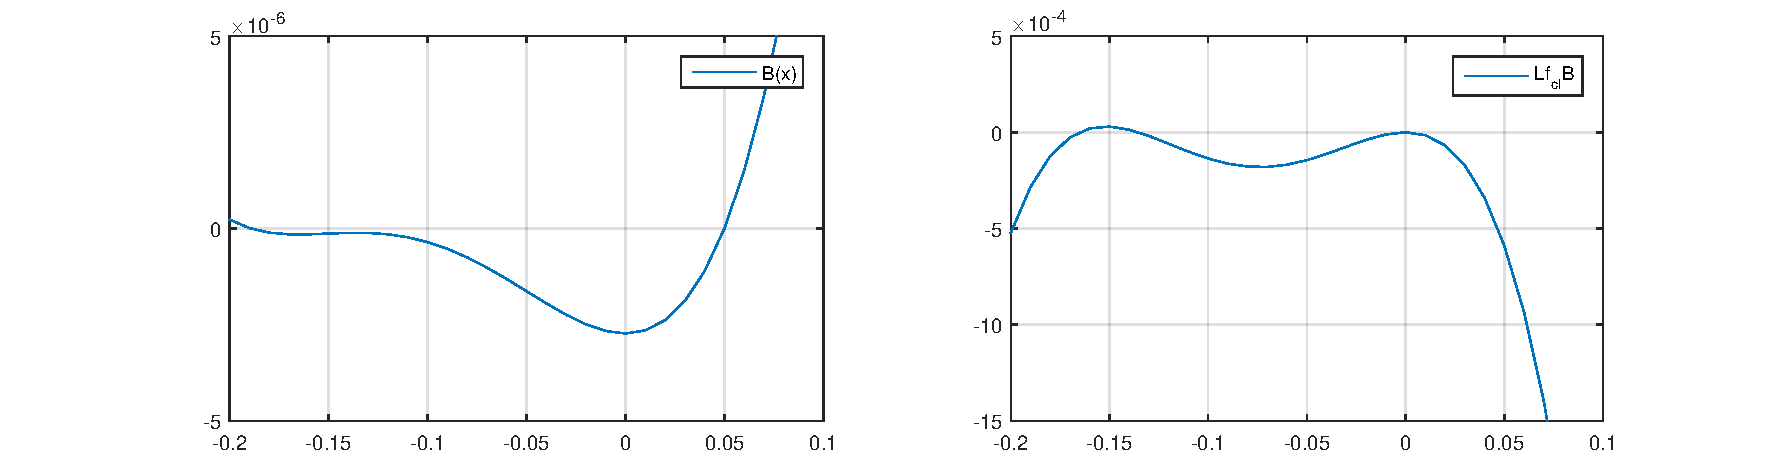
\includegraphics[width=1.1\textwidth]{1stordersys_staticlimits.pdf}
	\caption{A barrier certificate is found with SOSTOOLS that complies with the requirements in \autoref{eq:barrier_constraints}: it is positive on $\mathcal{X}_u=\{x_1\in [0.05\,\,0.1]\}$ and negative on $\mathcal{X}_0=\{x_1\in [-0.1\,\,0.05]\}$, and its Lie derivative is nonpositive on $\mathcal{X}=\{x_1\in [-0.1\,\,0.1]\}$.}
	\label{fig:barrier_1storder_staticlim}
\end{figure}

\section{Approach for Verification of System Safety}

The following chapters present the safety verification of first- and second order systems in 1D and 3D with static and dynamic boundaries using Putinar's Positvstellensatz in the SOSTOOLS framework. The same systems are used for the analysis as in \autoref{part:cbf}, and to the extent it is possible, also the same (pole placement design) controllers are tested. \textcolor{red}{Correct this when the chapters are written!!!}

